\documentclass[a4paper,parskip=half,ibliography=totocnumbered,titlepage]{scrartcl}

\usepackage[T1]{fontenc}  
\usepackage[utf8]{inputenc}
\usepackage[ngerman]{babel}
\renewcaptionname{ngerman}{\figurename}{Abb.}

\usepackage{multicol}         
\usepackage{mathtools}       
\usepackage{amssymb}
\usepackage{listings}      
\usepackage{csquotes}
\usepackage{pifont}

% Tabellen
\usepackage{booktabs}
\usepackage{multirow}
\usepackage{multicol}

\usepackage{tocloft}
\renewcommand{\cftfigpresnum}{Abb. }
\settowidth{\cftfignumwidth}{Abb. 10\quad}


\usepackage{ifthen}
\newcommand{\forloop}[5][1]{%
\setcounter{#2}{#3}%
\ifthenelse{#4}{#5\addtocounter{#2}{#1}%
\forloop[#1]{#2}{\value{#2}}{#4}{#5}}%
{}}

\newcounter{crcounter}

\newcommand{\compensaterule}[1]{%
\forloop{crcounter}{1}{\value{crcounter} < #1}%
{\vspace*{-\aboverulesep}\vspace*{-\belowrulesep}}}

\newcommand{\multirowbt}[3]{\multirow{#1}{#2}%
{\compensaterule{#1}#3}}


% bibtex
\usepackage[natbib,bibencoding=auto,style=authoryear,backend=biber]{biblatex}
\bibliography{references.bib}
\DeclareLanguageMapping{ngerman}{ngerman-apa}


%Schusterjungen und Hurenkinder
\clubpenalty = 10000
\widowpenalty = 10000

%Farbnamen benutzen
\usepackage[usenames,dvipsnames]{color}

\definecolor{black}{gray}{0} % Umdefinition der Farbe black, falls noetig (0=schwarz, 1=weiss)
\definecolor{dblue}{rgb}{0.1,0.2,0.6} % Dunkelblau, fuer Hyperlinks
\definecolor{lgray}{gray}{0.9} % Hellgrau, fuer Tabellen (0=schwarz, 1=weiss)
\usepackage[hyperfootnotes=false,colorlinks=true,linkcolor=black,citecolor=dblue,urlcolor=dblue]{hyperref} 

\usepackage{setspace}

\usepackage{enumitem}
\setlist{noitemsep} % or \setlist{noitemsep} to leave space around whole list

% \begin{enumerate}[label=(\roman{*})]

\newcommand{\HRule}[1]{\rule{\linewidth}{#1}} 	% Horizontal rule

\makeatletter							% Title
\def\printtitle{%						
    {\centering \@title\par}}
\makeatother									

\makeatletter							% Author
\def\printauthor{%					
    {\centering \large \@author}}				
\makeatother							

\usepackage{lastpage}
\usepackage{fancyhdr}
\pagestyle{fancy}
\fancyhf{}
\renewcommand{\footrulewidth}{0.5pt}
\renewcommand{\headrulewidth}{0.5pt}


% ------------------------------------------------------------------------------
% Metadata (Change this)
% ------------------------------------------------------------------------------

%Kopf- und Fußzeile, jeweils links und rechts
\fancyhead[L]{Dokumentation}
\fancyhead[R]{A.R.C.S.}
\fancyhead[L]{Projekt C}
\fancyfoot[R]{Seite \thepage\ von~\pageref{LastPage}}

%Titelblat
\title{\normalsize \textsc{Dokumentation Projekt C} 	% Subtitle of the document
		 	\\[2.0cm]													% 2cm spacing
            \HRule{0.5pt} \\ [0.5cm]										% Upper rule + 0.5cm spacing
			\LARGE \textbf{\uppercase{A.R.C.S - Android Rubik's Cube Solver}}	% Title
			\HRule{0.5pt} \\ [0.5cm]								% Lower rule + 0.5cm spacing
			\large Stephan Halbritter (Matr.-Nr.: 2093970)\\
      Colin Sames (Matr.-Nr.: 2093044)\\
		}

\author{Betreuer: Prof.~Dr.~Plaß\\
    Media Systems (B.Sc.)\\
    Hochschule für Angewandte Wissenschaften Hamburg\\
}


\begin{document}
% ------------------------------------------------------------------------------
% Maketitle
% ------------------------------------------------------------------------------
\thispagestyle{empty}				% Remove page numbering on this page

\printtitle									% Print the title data as defined above
  	\vfill
\printauthor								% Print the author data as defined above
\newpage

\begin{abstract}
Vermutlich brauchen wir hierfür kein Abstrakt, aber ich lasse es erstmal drin.
\end{abstract}

\tableofcontents
\newpage

\section{Idee}  % sgelb 90%
Die grundlegende Idee ist simpel und mit drei Schritten erklärt:

\begin{enumerate}

  \item Nehme einen ungelösten \emph{Rubik's Cube}

  \item Lese seine Seiten über die Kamera eines Smartphones ein

  \item Folge den Anweisungen und löse den Würfel

\end{enumerate}

Hauptaugenmerk lag hierbei auf dem möglichst einfachen Einlesen der sechs
Würfelseiten mit den insgesamt 54 Farbflächen.

\section{Der Würfel}  % sgelb

\begin{figure}[ht!]
  \centering
  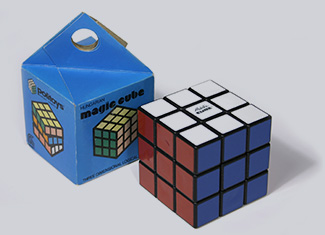
\includegraphics[width=\textwidth]{pics/rubikcube1977.jpg}
  \caption{Die ersten Exemplare wurden 1977 in Budapest verkauft
  (\cite{rubik:history})}
  \label{fig:rubik1977}
\end{figure}

Der \emph{Rubik's Cube} oder \emph{Zauberwürfel} wurde 1974 durch den
ungarischen Architekturprofessor Ernő Rubik erfunden, um seinen Studierenden
räumliche Verhältnisse anschaulicher präsentieren zu können. Seitdem beschäftigt
sich nicht nur die Mathematik immer wieder damit, der Würfel hat auch seinen
eigenen Sport, das \emph{Speedcubing} geschaffen.\footcite{rubik:history} 

\subsection{Aufbau}  % 100% sgelb

Der klassische sechsseitige Würfel aus Abbildung~\ref{fig:rubik1977} besteht aus
insgesamt 26 Teilen. Jede der sechs mittleren Flächen auf jeder Seite – die
\emph{Mittelteile} – hat eine eigene Farbe.\footnote{In der Regel sind dies
Orange, Blau, Rot, Grün, Weiß und Gelb} Sie lassen sich nicht rotieren, ihr
Position zueinander ist also festgelegt. Desweiteren gibt es zwölf
\emph{Kantensteine}, die zwei über eine Kante verbundene \emph{facelets}
verbinden und acht \emph{Ecksteine}, die drei \emph{facelets} über eine Ecke
verbinden.

\subsection{Lösungsalgorithmen}  % 0% sgelb

Insgesamt ergeben sich rund \( 4,3 \cdot {10}^{19} \) verschiedene
Kombinationen.

Lösungsansätze blabla, gewählt haben wir x weil y

\subsection{Notation}  % sgelb

F, R, B, L, D, U etc


\section{Umsetzung}  % sgelb 0%

\subsection{Bibliotheken und Tools}  % colin 0%
\subsubsection{OpenCV}  % 0%
\subsubsection{Eclipse}  % 0%
\subsubsection{Git}  % 0%
\subsubsection{ADT/NDK}  % 0%
\subsubsection{Java}  % 0%

\subsection{Gestaltung}  % sgelb 0%
\subsection{Arbeitsprozess}  % sgelb 0%

\section{Benutzerhandbuch}  % colin 0%

\section{Architektur}  % colin 0%
\subsection{Hierarchie}  % 0%
\subsection{Prinzipien}  % 0%

\section{Auswertung}  % sgelb 0%
\subsection{Ausblick}  % 0%
\subsection{Fazit}  % 0%


% Am Ende Bild- und Quellenverzeichnis
\appendix
\printbibliography[heading=bibintoc,title={Quellenverzeichnis}]
\listoffigures

\end{document}
